% Fraction-aware extension of the parent-only stationary theory.
\documentclass[10pt]{article}
\usepackage[margin=0.62in]{geometry}
\usepackage{amsmath,amssymb,booktabs,graphicx}
\usepackage[hidelinks]{hyperref}
\setlength{\parindent}{0pt}
\setlength{\parskip}{3pt}
\setlength{\abovedisplayskip}{4pt}
\setlength{\belowdisplayskip}{4pt}
\setlength{\textfloatsep}{7pt}
\setlength{\floatsep}{6pt}
\renewcommand{\arraystretch}{1.08}

\title{\vspace{-1.3cm}\textbf{Two-Block Circuit Competition with Neuron-Type Fractions}}
\author{}
\date{\vspace{-1.15cm}}

\begin{document}
\maketitle
\vspace{-0.75cm}

\textbf{Summary.}
We extend the parent-only stationary theory by allowing both $1+1\to2$ and
$1+1+1+1\to4$ neurons in block 1, and $1+1\to2$, $1+1+1+1\to4$, and
$2+2\to4$ neurons in block 2.  The raw-ReLU lower-mode byproducts are retained.  The central
result is slightly counterintuitive: with ordinary L2 weight decay and freely rescalable neuron
weights, the objective determines the \emph{aggregate squared norm carried by each circuit
family}, but not its literal fraction of neurons.  At zero temperature, the cheaper block-2
$d4$ family receives all block-2 target norm; it need not receive more neurons.  Positive
fractions only make routes available, while a zero fraction removes a route.  The enlarged
phase diagram follows from a five-order-parameter free energy.

\section*{1. Model, circuit populations, and assumptions}
For target parity $\chi_a(x)\in\{-1,+1\}$, let $f_a(x)=w_a^\top h_2(x)$ and
$\widehat A_a=\mathbb E[f_a\chi_a]$.  Under the aligned-mode ansatz,
$\mathbb E[(f_a-\chi_a)^2]=(1-\widehat A_a)^2$ because $\chi_a^2=1$.  We use
\begin{align}
h_1&=h_0+\sigma(V_1h_0),& h_2&=h_1+\sigma(V_2h_1),\nonumber\\[-5pt]
\mathcal J&=\frac{\gamma_2}{2}\!\sum_{a\in\{12,34\}}(1-\widehat A_a)^2
+\frac{\gamma_4}{2}(1-\widehat A_4)^2
+\frac12\!\left(\lambda_E\|E\|^2+\lambda_1\|V_1\|^2+\lambda_2\|V_2\|^2\right.\nonumber\\[-2pt]
&\hspace{5.0cm}\left.+\lambda_p\|W_{d2}\|^2+\lambda_4\|w_4\|^2\right).
\label{eq:objective}
\end{align}
The neuron fractions are
\begin{align}
&\rho^{(1)}_{2\times1}+\rho^{(1)}_{4\times1}+\rho^{(1)}_0=1,\nonumber\\[-2pt]
&\rho^{(2)}_{2\times1}+\rho^{(2)}_{4\times1}
+\rho^{(2)}_{2\times2}+\rho^{(2)}_0=1,
\qquad \rho^{(\ell)}_c\geq0,
\label{eq:fractions}
\end{align}
where $0$ denotes neurons not carrying one of the tracked circuits.  The subscripts mean,
respectively, $1+1\to2$, $1+1+1+1\to4$, and $2+2\to4$.

The coefficient bookkeeping comes directly from the balanced ReLU gates.  For signs
$\epsilon_i\in\{\pm1\}$,
\begin{align}
\sigma\!\left[a(\epsilon_1x_1+\epsilon_2x_2)\right]
&=\frac a2(1+\epsilon_1x_1+\epsilon_2x_2+\epsilon_1\epsilon_2x_1x_2),
\label{eq:d2-relu}\\
\sigma\!\left[a\sum_{i=1}^4\epsilon_ix_i\right]
&=a\!\left[\frac34+\frac12\sum_i\epsilon_ix_i
+\frac14\sum_{i<j}\epsilon_i\epsilon_jx_ix_j
-\frac14\Big(\prod_i\epsilon_i\Big)x_1x_2x_3x_4\right],
\label{eq:d4-relu}\\
\sigma[a(\chi_{12}+\chi_{34})]
&=\frac a2(1+\chi_{12}+\chi_{34}+\chi_{1234}).
\label{eq:compose-relu}
\end{align}
Thus a $2\times1$ gate has equal singleton and $d2$ magnitudes; a $4\times1$ gate whose
$d4$ magnitude is $r$ has singleton magnitude $2r$ and each pair magnitude $r$; and a
$2\times2$ gate has equal parent and $d4$ magnitudes.

We assume: (A1) the full four-bit cube and pure ReLU; (A2) equal-norm orthogonal modes within
each degree; (A3) sign-balanced populations, so the Walsh coefficient vectors produced by a
circuit family are mutually orthogonal; (A4) different circuit populations and the residual
embedding occupy orthogonal feature subspaces, so their squared norms add; (A5) sufficient
width and minimum-norm balanced gates; (A6) readouts align with the corresponding total mode
vectors; and (A7) the global zero-temperature minimum is reached.  A3--A4 are the closure that
makes neuron-level byproducts tractable.  Walsh orthogonality in function space alone would
not imply A4.

\section*{2. What the fractions do under standard weight decay}
Let $I_{\ell c}$ contain the $N_\ell\rho^{(\ell)}_c$ neurons assigned to circuit family $c$,
and let $u_j$ be the incoming-weight norm of neuron $j$.  Define
\begin{equation}
U_{\ell c}^2\equiv\sum_{j\in I_{\ell c}}u_j^2
=N_\ell\rho^{(\ell)}_c\,\overline{u^2}_{\ell c},
\qquad Q_{\ell c}^2=\eta_{\ell c}^2U_{\ell c}^2,
\label{eq:population-norm}
\end{equation}
where $Q_{\ell c}$ is the resulting mode-vector norm and $\eta_{\ell c}$ is the circuit
efficiency.  Eliminating the per-neuron scale gives
\begin{equation}
\frac{\lambda_\ell}{2}\sum_{j\in I_{\ell c}}u_j^2
=\frac{\lambda_\ell}{2\eta_{\ell c}^2}Q_{\ell c}^2,
\label{eq:fraction-cancels}
\end{equation}
which contains no $\rho^{(\ell)}_c$.  Equivalently,
$\rho^{(\ell)}_c\to a\rho^{(\ell)}_c$ and
$\overline{u^2}_{\ell c}\to\overline{u^2}_{\ell c}/a$ leave every retained mode and the L2
cost unchanged.  Therefore the fractions are flat directions whenever they are positive and
large enough to realize the balanced sign ensemble.  They cannot be fitted by minimizing
Eq.~\eqref{eq:objective}.  At finite width there is only a minimum-support/integrality
condition.  A per-neuron norm cap, fixed neuron norm, nonquadratic regularizer, or an explicit
entropy/dynamical model would be needed to predict literal counts.

The same argument distinguishes \emph{neuron fraction} from \emph{target-strength share}.
Let block 2 produce orthogonal target vectors of norms $Q_D,Q_C$ through its $4\times1$ and
$2\times2$ populations.  At fixed $Q^2=Q_D^2+Q_C^2$, their hidden cost is
\begin{equation}
\frac12(\kappa_DQ_D^2+\kappa_CQ_C^2)
=\frac{Q^2}{2}\big[(1-\alpha_C)\kappa_D+\alpha_C\kappa_C\big],
\qquad \alpha_C\equiv\frac{Q_C^2}{Q^2}.
\label{eq:strength-share}
\end{equation}
Consequently,
\begin{equation}
\alpha_C^*=\begin{cases}1,&\kappa_C<\kappa_D,\\0,&\kappa_C>\kappa_D,\\
\text{any value in }[0,1],&\kappa_C=\kappa_D.\end{cases}
\label{eq:winner-take-all}
\end{equation}
Thus the cheaper family carries all block-2 $d4$ norm at $T=0$; standard L2 decay does
\emph{not} say that it contains more neurons.  This winner-take-all result permits us to label
the two stationary families by $a\in\{D,C\}$.

\section*{3. Coupled mode geometry and the reduced free energy}
Retain the notation $s$ for the input singleton norm and $q$ for the block-1 parent norm
created by its $2\times1$ population.  Add $r$, the block-1 $d4$ norm created by its
$4\times1$ population; $p$, the extra parent norm created by block-2 $2\times1$ neurons; and
$Q$, the block-2 $d4$ norm carried by the winning $D$ or $C$ population.  Equations
\eqref{eq:d2-relu}--\eqref{eq:d4-relu} and A3--A4 give the singleton and canonical-parent norms
available at the input of block 2:
\begin{equation}
\boxed{S^2\equiv(Q_1^{(1)})^2=s^2+q^2+4r^2,
\qquad P^2\equiv(Q_{2,\mathrm{parent}}^{(1)})^2=q^2+r^2.}
\label{eq:SP}
\end{equation}
The $4\times1$ population also creates four cross-pair $d2$ modes of norm $r$.  If $q>0$,
the canonical parent pair has norm $P\geq r$ and is the cheapest compositional partition; at
$q=0$ the three partitions are degenerate and only add multiplicity, not a lower $T=0$ cost.

The minimum-norm identities used in the original derivation now apply to each population:
\begin{align}
\|E\|^2&=4s^2,&
\|V_{1,2\times1}\|^2&=\frac{16q^2}{s^2},&
\|V_{1,4\times1}\|^2&=\frac{64r^2}{s^2},\nonumber\\[-2pt]
\|V_{2,2\times1}\|^2&=\frac{16p^2}{S^2},&
\kappa_D&=\frac{64\lambda_2}{S^2},&
\kappa_C&=\frac{8\lambda_2}{P^2}.
\label{eq:costs}
\end{align}
For example, one first-block parent gate has efficiency $s/(2\sqrt2)$ and there are two
parents, while a first-block $4\times1$ gate has efficiency $s/8$; this produces the factors
$16$ and $64$.  Block-2 $2\times1$ neurons operate in parallel with the other block-2
neurons: they improve the parent readout but cannot become inputs to a $2\times2$ neuron in
the same block.

Both block-2 target circuits produce a canonical-parent byproduct of norm $Q$, by
Eqs.~\eqref{eq:d4-relu}--\eqref{eq:compose-relu}.  Hence the final norm available to each
parent readout and the final target-mode norm are
\begin{equation}
Z^2=q^2+r^2+p^2+Q^2=P^2+p^2+Q^2,
\qquad H^2=r^2+Q^2.
\label{eq:ZH}
\end{equation}
At fixed $(s,q,r,p,Q)$, minimizing over the common parent output amplitude $B$ and the $d4$
readout gives
\begin{equation}
B^*=\frac{\gamma_2Z^2}{\gamma_2Z^2+\lambda_p},\qquad
A^*=\frac{\gamma_4H^2}{\gamma_4H^2+\lambda_4},
\label{eq:amplitudes}
\end{equation}
and the two minimized loss-plus-readout terms are
$\gamma_2\lambda_p/(\gamma_2Z^2+\lambda_p)$ and
$\gamma_4\lambda_4/[2(\gamma_4H^2+\lambda_4)]$.  The complete phase-specific free energy is
therefore
\begin{align}
\mathcal F_a(s,q,r,p,Q)={}&2\lambda_Es^2
+8\lambda_1\frac{q^2}{s^2}+32\lambda_1\frac{r^2}{s^2}
+8\lambda_2\frac{p^2}{S^2}+\frac{\kappa_a}{2}Q^2\nonumber\\[-2pt]
&+\frac{\gamma_2\lambda_p}{\gamma_2Z^2+\lambda_p}
+\frac{\gamma_4\lambda_4}{2(\gamma_4H^2+\lambda_4)},
\qquad
\boxed{F_a=\min_{s,q,r,p,Q\geq0}\mathcal F_a},
\quad a\in\{D,C\}.
\label{eq:full-free}
\end{align}
This is one simultaneous minimization; the elimination order is only algebraic convenience.
The earlier parent free energy $\Phi(s,q)$ is no longer separable because $r$, $p$, and $Q$
all help the parent readout, while $r$ and $Q$ also help the $d4$ readout.  If block-1 $d4$
neurons and block-2 byproducts are projected out ($r=p=0$ and $Z=q$),
Eq.~\eqref{eq:full-free} reduces to the original $\Phi+G$ theory.

\section*{4. Phase boundary and the role of the fractions}
For a fixed learned representation $(s,q,r)$, Eq.~\eqref{eq:winner-take-all} selects composition
when
\begin{equation}
\kappa_C<\kappa_D
\quad\Longleftrightarrow\quad
\boxed{\frac{P}{S}>\frac1{\sqrt8}}
\quad\Longleftrightarrow\quad
\boxed{s^2<7q^2+4r^2.}
\label{eq:local-boundary}
\end{equation}
The block-1 $4\times1$ population can therefore improve compositional accessibility through
its $d2$ byproducts: its intrinsic squared parent-to-singleton ratio is $r^2/(2r)^2=1/4$,
above the required $1/8$.  But it simultaneously supplies a block-1 $d4$ shortcut, so the
global alternatives are
\begin{equation}
F_C<F_D\quad(2+2\to4\text{ in block 2}),\qquad
F_D<F_C\quad(4\times1\to4\text{ in block 2}),
\label{eq:global-boundary}
\end{equation}
together with a possible block-1-only solution $Q=0,r>0$, parent-only solution $A^*=0,B^*>0$,
or fully suppressed solution $A^*=B^*=0$.  The actual $C$--$D$ boundary is $F_C=F_D$ after
the two five-dimensional minimizations, not a comparison of target costs while holding the
other variables fixed.  Nevertheless, every strict global $C$ optimum must satisfy
Eq.~\eqref{eq:local-boundary}; otherwise changing only its block-2 target family to $D$ would
lower the same objective.

\begin{figure}[h!]
\centering
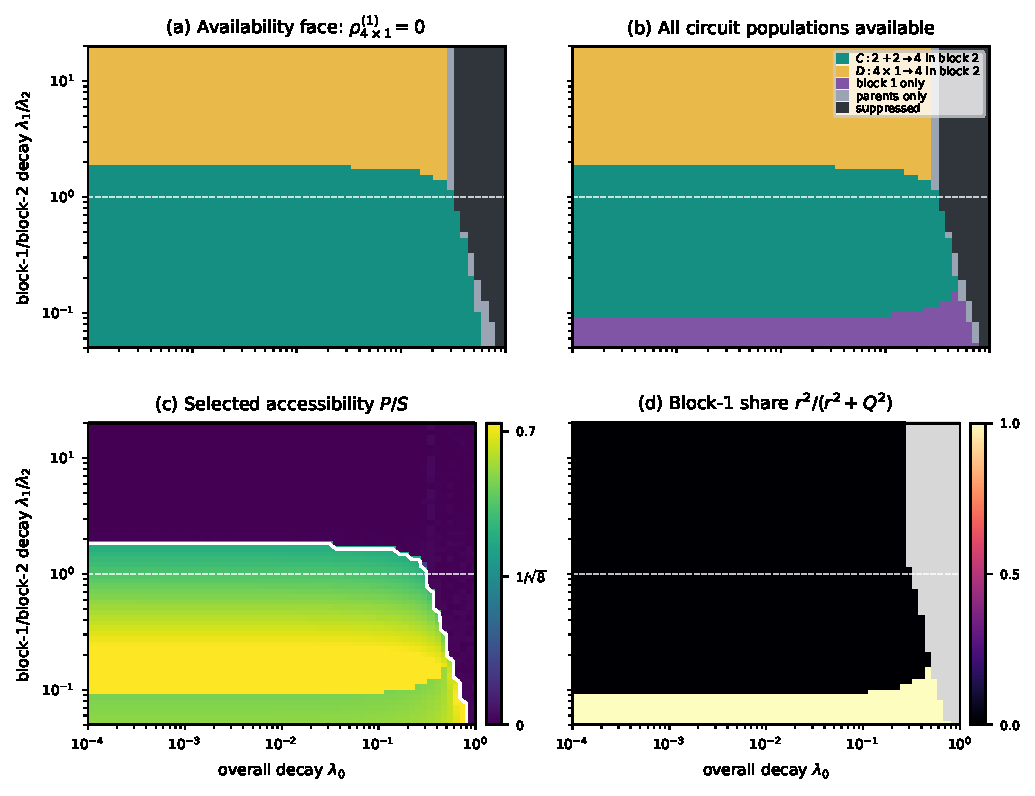
\includegraphics[width=0.77\textwidth]{fig_two_block_neuron_fraction_phase.pdf}
\vspace{-6pt}
\caption{\textbf{Canonical zero-temperature phase diagrams.}  We set
$\gamma_2=\gamma_4=2$, $\lambda_E=\lambda_p=\lambda_4=\lambda_2=\lambda_0$, and vary
$\lambda_1/\lambda_2$.  (a) Equation~\eqref{eq:full-free} on the availability face
$\rho^{(1)}_{4\times1}=0$.  (b) Its minimum when every population in
Eq.~\eqref{eq:fractions} is available.  (c) Selected accessibility $P/S$; the white contour is
$1/\sqrt8$.  (d) The aggregate block-1 share of hidden $d4$ squared norm, not the neuron
fraction.  Gray means the target is suppressed.  The occupied-model diagram is invariant
under all strictly positive values of the $\rho$'s: only setting a fraction to zero changes the
allowed minimization domain.  The diagrams are numerical global-search approximations to the
displayed reduced free energies.}
\label{fig:phase}
\end{figure}

\textbf{Answers and control implications.}
The first-block strengths $(q,r)$ and second-block strengths $(p,Q)$ are determined by
Eq.~\eqref{eq:full-free} (up to phase-boundary degeneracies), but the neuron fractions are not.
No empirical fraction needs to be fitted to obtain the standard-WD energy phase diagram if all
families are available; conversely, this theory cannot predict observed neuron counts.  The
sharp zero-temperature prediction for block 2 concerns $\alpha_C$, not
$\rho^{(2)}_{2\times2}$.  To favor $2+2\to4$, preserve enough canonical-parent strength that
$P/S>1/\sqrt8$, keep $\lambda_2\lambda_4$ low enough that the target is not suppressed, and
avoid making block 1 so cheap that it solves $d4$ by itself.  Layerwise decay can move all
three quantities self-consistently, so the reliable criterion remains the full comparison
$F_C$ versus $F_D$.  Beyond this closure, overlaps give Gram forms and finite width or
cancellation costs add order parameters.  Finite temperature can lift flat fraction directions
only after a microscopic measure is specified.

\end{document}
